\documentclass[12pt]{report}

%% Language and font encodings
\usepackage[english]{babel}
\usepackage[utf8]{inputenc}
\usepackage[T1]{fontenc}
\usepackage{lscape}
%\usepackage{subfigure}
%% Sets page size and margins
\usepackage[a4paper,top=3cm,bottom=3cm,left=3cm,right=3.5cm,marginparwidth=1.75cm]{geometry}
\usepackage{fancyhdr}
\renewcommand{\baselinestretch}{1.5}

\newcommand{\HRule}{\rule{\linewidth}{0.5mm}}
\newcommand\frontmatter{%
    \cleardoublepage
  %\@mainmatterfalse
  \pagenumbering{roman}}

\newcommand\mainmatter{%
    \cleardoublepage
 % \@mainmattertrue
  \pagenumbering{arabic}}


\pagestyle{fancy}
%%

%% create an alias for \mathbf{}
\newcommand{\myvec}[1]{\mathbf{#1}}

\usepackage{gensymb}
\usepackage{mathtools}
\usepackage{todonotes}
\usepackage{biblatex}
\usepackage{graphicx}
\usepackage{caption}
\usepackage[justification=centering]{subcaption}
\addbibresource{references.bib}

\begin{document}

\begin{titlepage}
\begin{center}
\textsc{\LARGE Università di Pisa}\\ % University name
Dipartimento di Ingegneria dell'Informazione\\
Corso di Laurea Specialistica in Computer Engineering\\[1cm]
\begin{figure}[h]
\centering

\includegraphics[scale=0.5]{img/Unipi_logo}
\end{figure}

\textsc{\Large Laurea Specialistica in Computer Engineering}\\[0.5cm] % Thesis type

\HRule \\[0.4cm]
{\huge \bfseries 3D Environments Reconstruction using 360 Videos}\\[0.1cm] % Thesis title
\HRule \\[1cm]
 
\begin{flushleft} \large
\emph{Supervisors:}\\
Marco AVVENUTI\\
Francesco BANTERLE \\
Massimiliano CORSINI% Supervisor name - remove the \href bracket to remove the link  
\end{flushleft}

\begin{flushright} \large
\emph{Candidate:}\\
Andrea BECONCINI\\[1.5cm] % Author name - remove the \href bracket to remove the link
\end{flushright}
 
% \large \textit{A thesis submitted in fulfilment of the requirements\\ for the degree of \degreename}\\[0.3cm] % University requirement text
% \textit{in the}\\[0.4cm]
% \groupname\\\deptname\\[2cm] % Research group name and department name
 
{\large Academic Year 2016-17}\\[4cm] % Date
%\includegraphics{Logo} % University/department logo - uncomment to place it
 
\vfill
\end{center}

\end{titlepage}

\fancyhead[L]{\slshape \leftmark}
\fancyhead[R]{}

\frontmatter


\fancyhead[L]{\slshape \leftmark}
\fancyhead[R]{}

\frontmatter
\begin{abstract}
\thispagestyle{plain}
\addcontentsline{toc}{chapter}{Abstract}
360\degree degrees or full spherical images are gaining a huge interest in different fields such as, autonomous driving, cinematography, augmented reality (AR), and virtual reality (VR).

Computer vision research addressing spherical images is less popular than the one that considers traditional perspective cameras. However, this new kind of  devices allow users to capture an entire environment in a single shot.

In this work, we developed a structure from motion (SfM) pipeline for full spherical cameras composed of two main parts: camera poses estimation, and dense point cloud reconstruction. This pipeline employs frames captured using a 360\degree video-camera in the  equirectangular format.

Our contribution includes: a visual-based frame filter that selects frames to be used for motion estimation, a novel SfM pipeline implementation in MATLAB, and an adaptive window matching 
procedure for point cloud densification.

We tested the performance of our work both with a synthetic 3D scenes and with real sequences captured with a Ricoh Theta S camera.
\end{abstract}


\setcounter{page}{2}
\pagestyle{fancy} % The page style headers have been "empty" all this time, now use the "fancy" headers as defined before to bring them back
\addcontentsline{toc}{chapter}{Contents}
\lhead{\emph{Contents}} % Set the left side page header to "Contents"
\tableofcontents % Write out the Table of Contents
\cleardoublepage

\mainmatter
\chapter{Introduction}
\lhead{\chaptername~\thechapter. \emph{Introduction}}
The growing interest of the general public in spherical cameras technologies, which were 
research-only exclusives once, has made them less expensive and more available. For example, omindirectional cameras by GoPro have been extremely popular amongst sports men who publish them on social networks.

These devices have been employed in robotics since their first appearance to help navigate the robot in a real-world environment, and nowadays for autonomous driving. Furthermore, they can be exploited to deliver a virtual or augmented experience for augmented and virtual reality (AR/VR).

In this work, we designed a \textit{structure from motion} (SfM) pipeline for 
full spherical cameras. SfM is a well known topic in computer vision; it addresses the problem of 
recovering the structure of 3D environments from a sequence of images taken from different views.

SfM research (and computer vision in general) has targeted perspective cameras because these type of devices have always been more common. However, the increase of interest around these cameras has started a shift of interest towards employing them for research.

\begin{figure}[htb]
	\centering
    %
	\begin{subfigure}{0.4\textwidth}
		\centering
		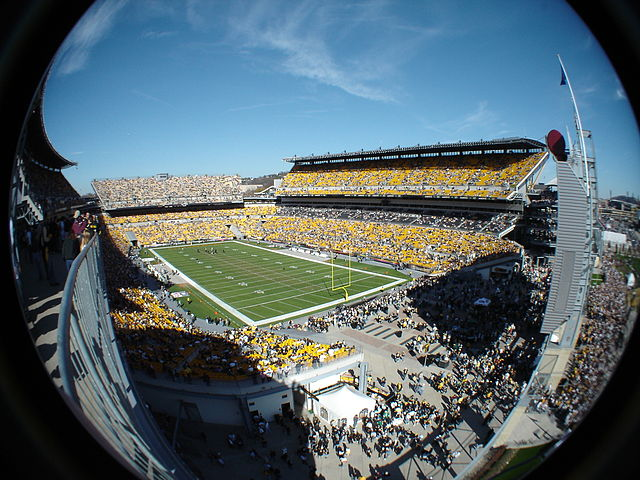
\includegraphics[width=\textwidth]{img/fisheye_example}
		\caption{Fisheye.}
        \label{fig:fisheye_example}
	\end{subfigure}
    %
	\begin{subfigure}{0.4\textwidth}
		\centering
		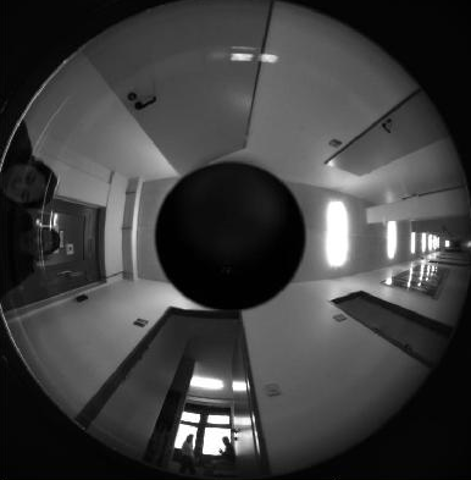
\includegraphics[width=\textwidth]{img/omnidirectional_example}
		\caption{Ominidirectional (catadioptric).}
        \label{fig:omnidirectional_example}
	\end{subfigure}
    %
	\caption{Some examples of fisheye pictures.}
    \label{fig:wide_fov_pics}
\end{figure}

\section{Omnidirection Cameras}
Large field of view (FOV) photography employs fisheye lenses that are capable to cover 
wider scene compared to traditional cameras' hardware.
The applications for this kind of equipments range from architectural or 
landscape photography to academic use for studies related to astronomic, 
meteorology, computer graphics, etc.
Photographers can also choose fisheye lenses for the characteristic distortion
these devices introduce and that provides more importance to foreground objects
(see Figure~\ref{fig:wide_fov_pics}~(\subref{fig:fisheye_example}) for an 
example of a picture taken with fisheye lenses equipped camera).
An example of wide FOV photography equipment is the GoPro\registered's camera series.
GoPro Inc\registered. produces action cameras, small digital devices for recording videos 
and taking pictures in harsh environments; their products have gained quite 
some success among the consumer market, also thanks to their marketing campaign 
that successfully associated their product to extreme sport events.
Action cameras like GoPro\registered's exploit wide FOV lenses that help to capture larger
scenes and make the devices fit to be worn.

Apart of wide FOV hardware there is another class of  
cameras that take panoramic photography to a new level: 
the 360\degree full spherical devices, capable of capturing images
in every directions with no blind sides. This class of devices employs 
several image sensors and integrated stitching software to automatically produce
panoramic pictures. This is the case for the Ricoh Theta S\texttrademark 
\cite{theta_website} we used in this work (Figure~\ref{fig:ricoh_theta}).

\begin{figure}[htb]
	\centering
	\begin{subfigure}{0.3\textwidth}
		\centering
		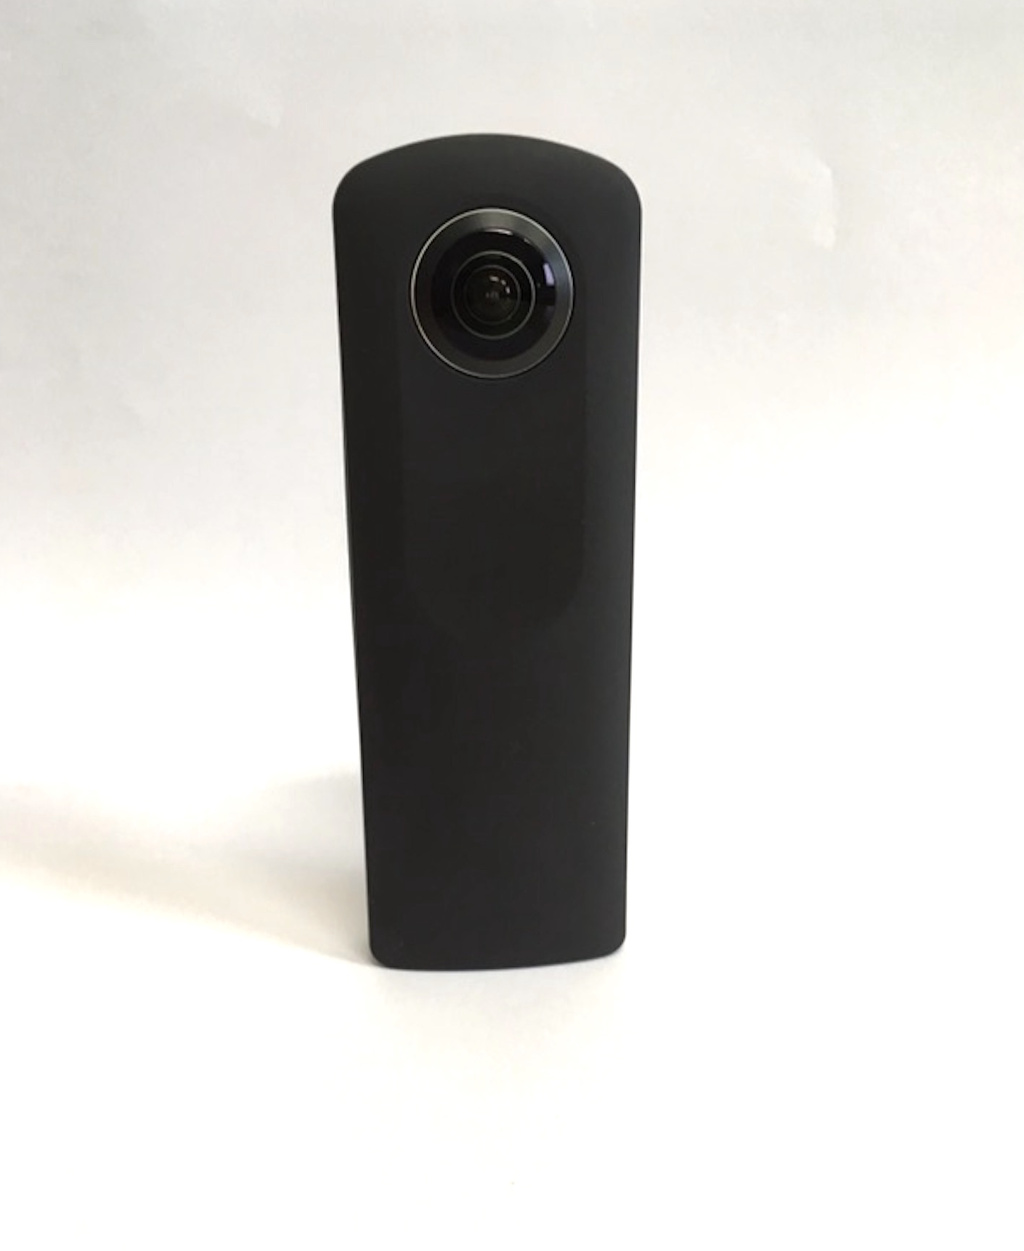
\includegraphics[width=\textwidth]{img/theta1}
	\end{subfigure}
    %
	\begin{subfigure}{0.3\textwidth}
		\centering
		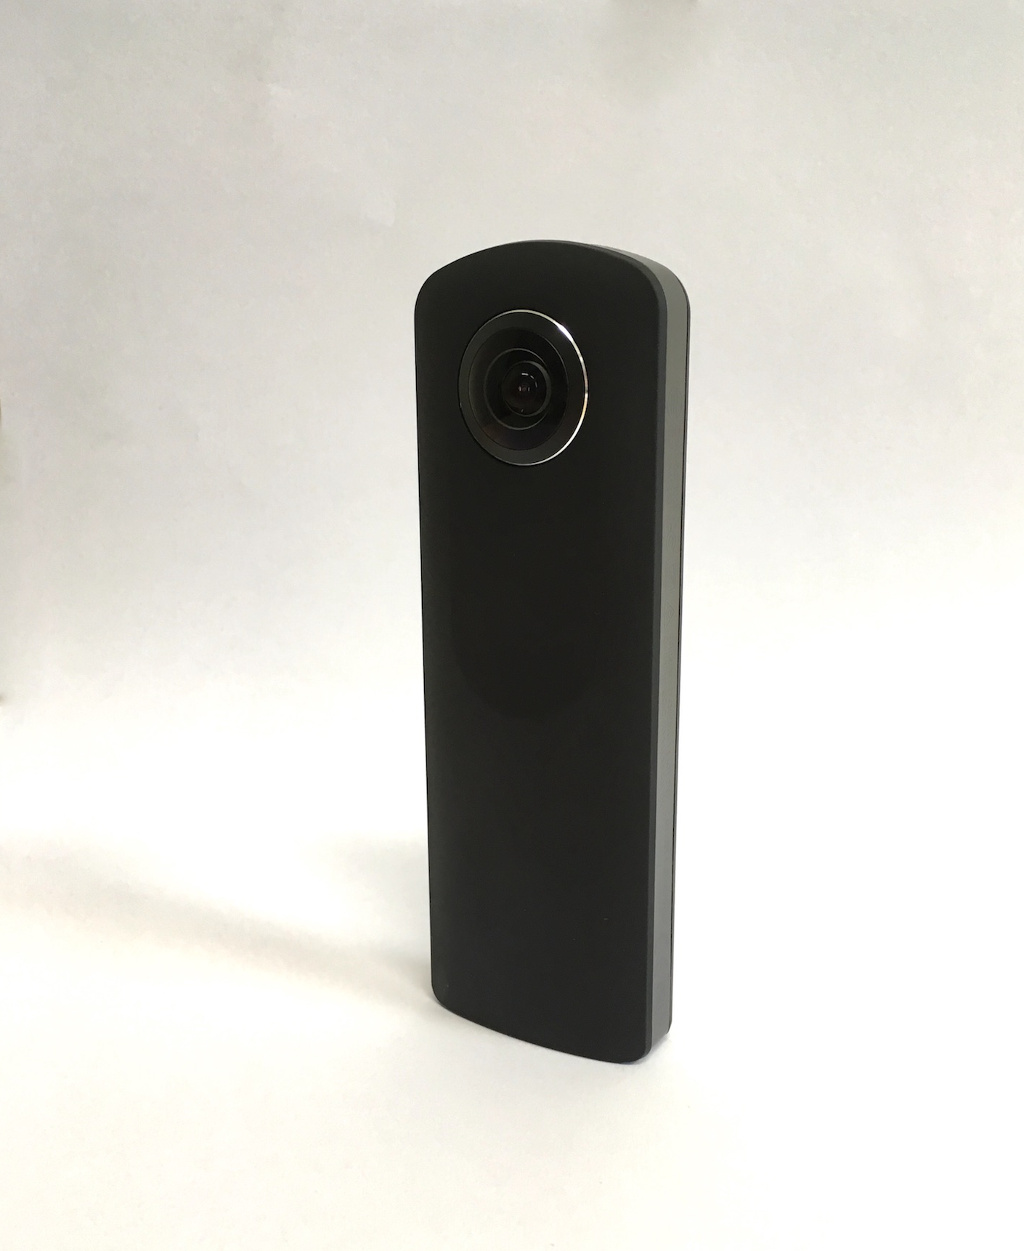
\includegraphics[width=\textwidth]{img/theta2}
	\end{subfigure}
    %
	\begin{subfigure}{0.3\textwidth}
		\centering
		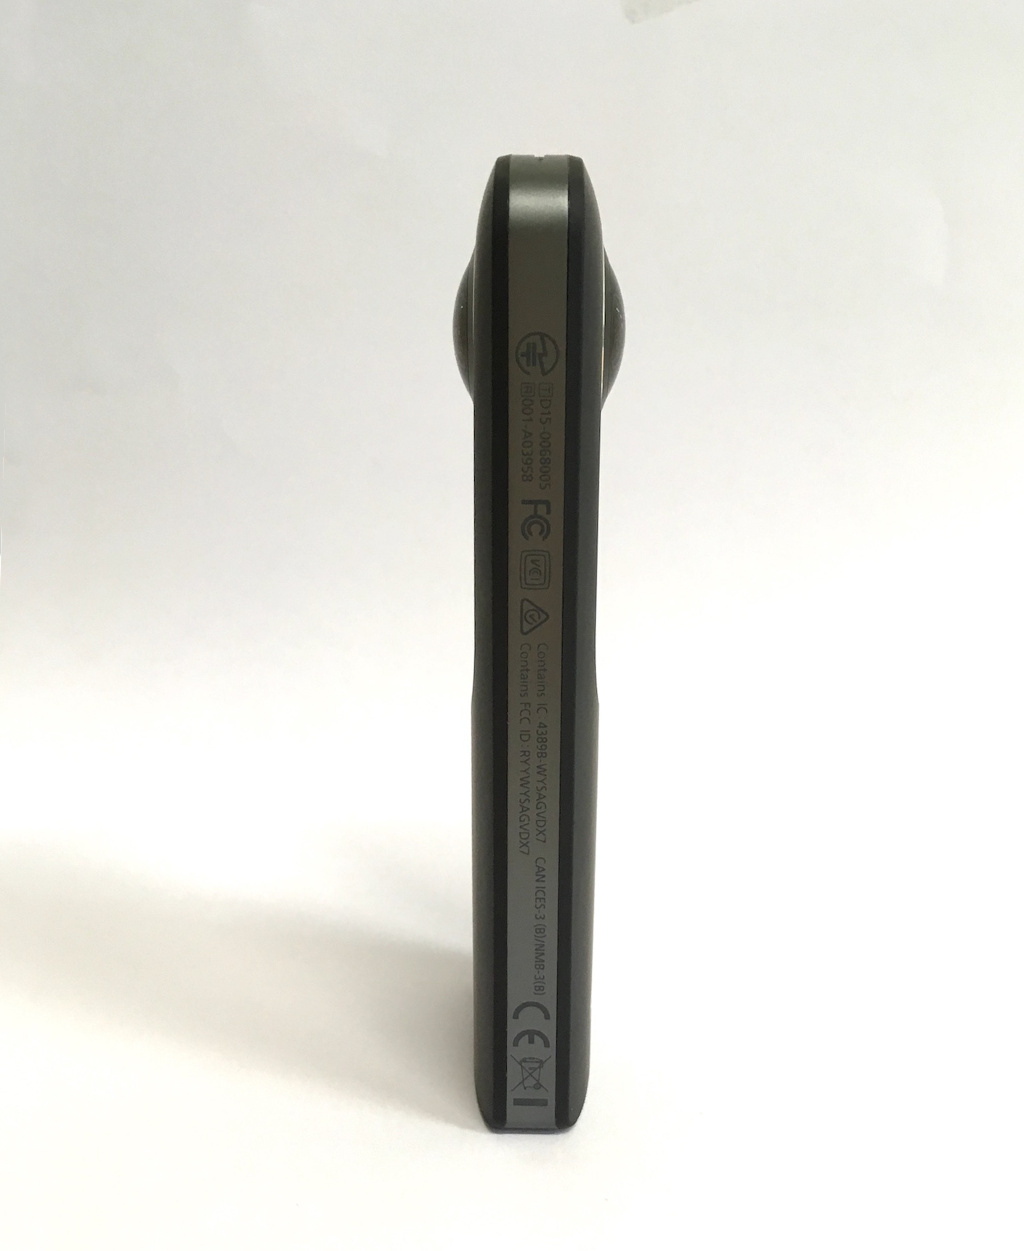
\includegraphics[width=\textwidth]{img/theta3}
	\end{subfigure}
    %
	\caption{The Ricoh Theta S\registered 360\degree camera.}
    \label{fig:ricoh_theta}
\end{figure}

Together with consumer hardware, some off-the-shelf
solutions for the professional market have started to appear. They include the Insta360
Pro\registered that can capture full spherical videos or pictures
at 8K resolution.
Another example is the GoPro Omni\registered. This camera is a simple 
rig that contains 6 traditional GoPro\registered devices that comes with 
specialized software to enables the 360\degree videos creation. Note that the interest in full spherical media creation is driven by the introduction of new immersive media fruition devices such as \textit{head-mounted display} (HMD); e.g. the Oculus Rift, the HTC Vive, the Sony PlayStation VR, etc.

\section{SfM Applications}
SfM is a well known topic in the computer vision community; it started after 
the landmark papers by Longuet-Higgins \cite{longuet1981computer} and
Nister et al. \cite{moravec1980obstacle}.
The problem can be described as the reverse of image formation
\cite{Wei2013}, as it targets the reconstruction of the environment 
and camera poses given a set of two or more images.
Some of the first application for this technology included robotic research, 
like navigation systems intended for rover explorations 
\cite{moravec1980obstacle,durrant1996localization}. In fact, NASA has supported
many researches because of the need for navigation systems not affected by wheels
slippage on uneven terrains.
SfM is used in geographical data acquisition too
\cite{fonstad2013topographic, westoby2012structure, james2012straightforward}
as alternative to other methods that employ specialized hardware and are generally more expensive.
Furthermore, there are applications for cultural heritage conservation because 
environment reconstructions can help in case of restoration of historical finds
\cite{kraus2007photogrammetry}.
Finally, the game industry is yet another field that can benefit from 
SfM: real environments can be reconstructed with SfM first and then 
improved by artists. Some game engine, as the popular Unreal Engine\registered,
includes photogrammetry software that exploits SfM techniques. \todo{non ho trovato un riferimento}
\todo[inline]{chiedere per un esempio di foto fisheye}

\chapter{State of the Art}
\lhead{\chaptername~\thechapter. \emph{State of the Art}}
\label{ch:state_of_the_art}
In this chapter we give a formal definition of the VO problem, we describe a 
general perspective SfM pipeline, then 
we explain the fundamental challenges issued by the employment of full 
spherical cameras for VO.

\section{VO Problem}
\label{sec:vo_problem}
As we described in the previous chapter, the VO's goal is to recover the 
camera trajectory while it is moving in the environment. We now
introduce the notations we are going to use for the rest of this work; 
these are the same ones used by Scaramuzza in \cite{scaramuzzaVisualOdometryI}.
Let first assume time is sampled in a sequence of time instants \(k\); 
\(I_{0:n} \) is the set of input frames, with \(I_{k}\) the picture taken by 
the camera at time
\(k\). We define \(C_{0:n}\) as the set of camera 
positions such that \(C_k\) is the position at the \(k\)-th instant.
If we call \(T_k\) the rigid body transformation of the camera between the two
consecutive time instant $k-1$ and $k$, then we have the following relation:
\begin{equation}
	\label{eq:motion_composition}
C_n = C_{n-1} T_n
\end{equation}
\noindent with \(T_k\) defined as
\begin{equation*}
	T_k =
	\begin{bmatrix}
	R_k & \myvec{t}_k \\
	0 & 1
	\end{bmatrix} \text{.}
\end{equation*}
\noindent $R_k$ is a 3-by-3 rotation matrix while $\myvec{t}_k$ is a column vector, 
they represent the rotation and translation the camera performed from instant 
$k-1$ to $k$.
Therefore the goal of VO is to estimate both $R_k$ and $t_k$ for each instant 
$k$ and then compute the camera position $C_k$ accordingly to 
equation~\ref{eq:motion_composition}.
The initial position $C_0$ can be set arbitrarily.

Equation~\ref{eq:motion_composition} is the core of VO: thanks to it we are able
to compute the camera local movement, therefore we can estimate its location in 
every moment. But the equation above contains also the biggest practical 
challenge of VO, that is the error accumulation phenomenon known as 
\textit{drift}.
Every new position $C_k$ introduces an error factor that affects the next 
computations; the results is a global error that grows as the number of 
estimations increases.
All the efforts of the VO research community since early works like 
\cite{harris19883d} and \cite{moravec1980obstacle}, has focused on error
minimization techniques to reduce drift.
These tackle the precise estimation problem either by employing more accurate
local motion estimation and by introducing an optimization step to refine 
camera locations.
The set of techniques by which the drift is reduced once the camera poses have 
have been computed go under the general term \textit{bundle adjustment}.

\section{Perspective SfM}
The SfM literature is extensive but most of the approaches the 
researches followed so far present pipelines similar to the one in 
Fig~\ref{fig:block_diagram}.
The main steps of the : compute the relative motion for each image
pair, then compose these motions to obtain the absolute camera position and 
orientation. Finally, run an optimization procedure to reduce drift.
The differences are in the type of input data, motion estimation algorithm,
optimization procedure and additional constraints considered.
For generic SfM researches, the input data is a set of traditional pictures of 
the same environment from different point of view. The pictures can be taken by 
different cameras with unknown parameters and in different time instants.
\begin{figure}
	\label{fig:block_diagram}
   \centering
    \def\svgwidth{0.5\columnwidth}
    \input{img/block_diagram.pdf_tex}
    \caption{Perspective SfM pipeline block diagram.}
\end{figure}
\textit{Visual Odometry} is based on SfM techniques, 
in this case, the input data is usually a sequence 
of images from a video stream. Many studies targeted different hardware setup 
but the specific image capturing device is usually either a single perspective 
camera or a stereo imaging rig. The computer vision literature refers to the
former case with the term \textit{monocular VO} while it uses \textit{stereo VO}
to describe the latter.

Even though perspective cameras have been the first choice in many studies, 
the researchers used other devices, like the ones described in 
\ref{sec:cameraclassification}.

We use the terms \textit{perspective} or \textit{traditional SfM} to describe 
SfM pipelines designed for perspective cameras.

A great resource about the state of the art for Visual Odometry and Structure 
from Motion techniques is the couple of articles by Scaramuzza,  
\cite{scaramuzzaVisualOdometryI} and \cite{scaramuzzaVisualOdometryII}.

\subsection{Motion Estimation}
We use the term local motion to indicate the camera movement between two 
consecutive images while, on the other hand, we define global motion as
the overall camera's path.
The local motion estimation step is fundamental in a SfM pipeline, its goal is 
to find the rigid body transformation composed of $R_k$ and $t_k$ as we 
described in Section~\ref{sec:vo_problem}.
All the local motion estimation methods described in the literature so far are 
based on the correspondences found in two consecutive images but, depending on the
specific camera rig (stereo imaging systems or monocular), the type of 
correspondences and their matching procedure, we may have several choices for
the actual way to estimate local motion.
There are two main families of point matching algorithms: \textit{feature-based}
and \textit{appearance-based} (also known as \textit{global-methods}).
While the former ones utilize repeatable features 
matching between the images, the latter rely on pixel's intensity information; 
they are simpler but also slower. Most of the 
most recent VO pipelines use feature-based methods because of
their speed and robustness.
A VO implementation that employs intensity based techniques is 
\cite{nister2004visual}, while ...\todo{aggiungere qualche citazione che non usi approcci misti}

Each of the feature points found by the motion estimation phase can be 
either a 3D world-point feature or a 2D image-point one,
therefore, there are three possible combinations that provides just as many 
different matching and motion-estimation procedures:
\begin{itemize}
	\item 2D-to-2D: both feature sets are composed of image points.
The matching metric can be a simple euclidean distance between feature 
descriptors and the motion estimation can be solved by estimating the 
\textit{essential matrix} (see section~\ref{subsec:essential_matrix} for 
details);
	\item 3D-to-3D: both feature sets contain world-points features and motion
estimation is performed by solving an alignment problem;
	\item 3D-to-2D: the previous image's feature set is composed of world points while
the current one's feature set contains their projections. In this case, the motion 
is estimated by solving a \textit{PnP} problem.
\end{itemize}
Since the second and third approaches deal with 3D points, they are usually 
best suited for stereo rig (especially the 3D-to-3D case).
Yet we can still use the 3D-to-2D approach in the monocular VO case by simply 
triangulating corresponding 2D image features in consecutive frames.
In fact, in order to obtain the first 3D feature set,
we can compute the relative motion between the first two images with 
the 2D-to-2D techniques and then obtain the rest of the camera's path,
as we said, by solving the \textit{PnP} problem.

\subsubsection{Essential Matrix}
\label{subsec:essential_matrix}
The essential matrix $E$ is defined by the equation
\begin{equation}
\label{eq:epipolar_equation}
\mathbf{p}'^\top E \mathbf{p} = 0
\end{equation}
\noindent where $\mathbf{p}$ and $\mathbf{p}'$ are the normalized corresponding 
feature coordinates in the image $I_{k-1}$ and $I_{k}$ respectively.
The normalized coordinates are defined as:
\begin{equation}
	\mathbf{p} = K^{-1} \mathbf{m}
\end{equation}
\noindent where $K$ is the intrinsic parameter matrix and $\mathbf{m}$ is an
image point.
The essential matrix contains the geometric information that describe the 
relative location of a camera respect to another one up to an unknown scale factor 
for the translation vector. In particular, we have
\begin{equation*}
	E_k = \lambda \hat{t}_kR_k
\end{equation*}
\noindent with $\lambda$ that is the unknown scale factor and $\hat{t}_k$ is 
the skew-symmetric form for the cross product of vector $t_k$.
In order to extract the local motion given the two set of corresponding features
in two consecutive images, we have to estimate the essential matrix and then 
extract the rigid body transformation out of it.
For the $E$ estimation part we can employ the Longuet-Higgins' 8-points 
algorithm \cite{longuet1981computer}: the equation~\ref{eq:epipolar_equation} 
provides a constraint we
can exploit for computation, in fact, for each correspondence, we can rewrite 
the equation as
\begin{equation*}
	\begin{bmatrix}
		p_1p'_1 & p'_1p_2 & p'_1 & p_1p'_2 & p_2p'_2 & p'_2 & p_1 & p_2 & 1
	\end{bmatrix}
	E = 0	\text{.}
\end{equation*}
To find the nine unknowns we need 8 noncoplanar feature matches that provide as many 
independent equations.
In practice we use more than 8 points, therefore we obtain a overdetermined 
system we solve in the least square sense.

Once $E$ has been estimated, there are 4 possible combinations for the relative 
position of the two cameras and each world points. We are interested in the one
that presents both cameras facing toward the triangulated world point,
i.e. this point has to be in front of both cameras. We can easily chose the 
correct configuration among the four by testing each of them.

\subsubsection{Relative Scale}
As we have already pointed out in the previous section, every monocular SfM 
pipeline that works with 2D-to-2D feature correspondences can estimate the 
local motion up to an unknown scale factor. In fact, there is no way to extract 
the translation magnitude from two sets of features (it is still possible 
to recover the reconstruction scale if we are given some world measure of the
environment).
Therefore, if we can not derive the local translation length with some other
non visual techniques (like wheel odometry, GPS, accelerometer, etc.), 
all we can do is to leave the unknown scale for the motion estimation and 
environment reconstruction.

On the other hand, if we have to compose the motion of more than two poses, 
like VO does, we need to set the first local translation magnitude 
arbitrarily and express all the other movements relative to this first one.
This means that we need to compute the \textit{relative scale}
for every translation other than the first one.

A possible approach for relative scale estimation is described in 
\cite{scaramuzzaVisualOdometryI}. If we want to estimate the relative scale for 
the motion $t_k$, between instants $k-1$ and $k$, we need to compute the 
two sets of triangulated world points $X_{k-1}$ and $X_{k}$ by using 
the two image pairs $I_{k-2}$ and $I_{k-1}$ , and  $I_{k-1}$ and  $I_{k}$ first; then,
given $i$ and $j$, two world points that belongs to both sets $X_{k-1}$ and 
$X_{k}$, we can compute the relative scale accordingly to these points with
\begin{equation}
	\label{eq:relative_scale}
	r = \frac{\| X_{k-1, i} - X_{k - 1, j} \|}{\| X_{k, i} - X_{k, j} \|}
	\text{.}
\end{equation}
\noindent For each world points pair, we obtain a different values of $r$;
we can then select the average of $r$ (or better, its median in case of 
outliers).

It is worth noticing that the exact \textit{absolute scale} for the whole 
camera motion and environment reconstruction is still left unknown.

\section{Full Spherical Cameras}
\subsection{Image Format}
If we consider the simplest camera model, 
a perspective image is the result of the intersection between the image plane 
and all the light rays that go from the environment to the center of 
projection inside the camera (see Fig\ref{fig:perscam_model}).
\missingfigure{aggiungere modello camera prospettica}
\label{fig:perscam_model}
On the other hand, the full spherical camera model implies the image plane 
to be the result of the intersection between a sphere and the rays from the 
environment to the center of projection (which is equivalent to the sphere's 
center).


\chapter{Spherical SFM}
\todo[inline]{aggiungere una sessione in cui si descrive il sistema di riferimento e 
altre convenzioni}
\section{Overview}
We now describe the pipeline we designed to create a dense point cloud from 
a set of equirectangular images.

The pipeline is composed of two main parts: an initial camera poses estimation
step followed by a densification phase. The former aims to reconstruct the 
camera trajectory, which means to estimate the camera position for each frame 
considered. The latter one relies on the previous result to create a dense 
3D point cloud that represents a simple reconstruction of the environment.
The Figure (...) is a simple visualization of this two macro parts of the 
pipeline.

The camera poses estimation phase is similar to other classical visual 
odometry pipeline; the real differences lie in the variables format and in 
the details concerning the procedures used. For each new frame 
(in the equirectangular format), we locate the
SURF keypoints; we consider those keypoints whose inclination angle belongs 
to the range [-60\degree; +60\degree] because the poles are affected by great 
distortions, thus robust matches outside this interval are rare.
Then we look for matches in the last two frames and a filter performs some 
statystical analysis on the correspondances found and decides whether the frame 
is suitable for a robust pose estimation or not (in which case the frame is 
discarded).

If the frame is kept, its matches with the previous one are converted
and used for the essential matrix estimation. Once E has been obtained, 
it can be decomposed in the \([R|t]\) form where R is a rotation matrix 
and t is a translation vector up to an unknown scale factor.

The relative scale can be estimated thanks to the world points which have been 
triangulated thorough the matches and frame considered in previous pipeline 
iteration.

The pose for each camera can then be described as the composition of the 
motions between each view pair. We perform a bundle adjustment for the last 5 
poses in order to reduce the effect of drift.

Once every image has been processed by the visual odometry pipeline, a final 
bundle adjustment is run. It optimizes every camera pose estimated in order to 
further reduce drift error.

In the following sections we describe every detail of the steps in our pipeline.

\section{Key Points and Features extraction}
In this step, we extract SURF key points and their descriptor out of 
equirectangular images. SURF 
interest points are rotation and scale invariant just like SIFT. But unlike 
the latter, SURF detection is faster and there is no patent for it. 
This makes SURF implementation available in most computer vision frameworks and 
libraries.

\section{Key points filtering}
The equirectangular format for spherical images introduces significant 
distortions in the areas around the poles. Interesting points in those areas 
are unlikely to match reliably with other points in a consecutive view, 
so they are just discarded.

Besides, in our experiments setup, the north and south poles usually point 
upward and downward respectively while most of the matches useful for pose 
estimation comes from the sides of the camera, so the removal of interesting 
points near the poles does not really affect the final result.

\section{Feature matching}
The matching strategy we carried out for equirectangular images is the same one 
adopted with standard images: two key points matches if the distance between 
their descriptors is less than a given threshold. Ambiguous matches 
are discarded if the ratio between the distances to the two closest matches is 
above a maximum.

We enforce matching robustness by forcing unique matching, that is: a feature 
in an image can possibly match to one feature only in the other image.
This is obtained with a first former forward matching followed by a backward 
pass that, in case of multiple matches, selects the best one only.

\section{Matches filter}
In this step of the pipeline the matches are analyzed in order to decide 
whether a frame is kept because it is useful for motion estimation or 
it has to be discarded.

We assume the environment considered for our studies is static: no people, 
cars or any kind of moving object is present in our scene. In this case the 
apparent movement of corresponding objects in different views is caused by 
the camera motion only. This hypothesis simplifies the pipeline and, 
in particular, provides some hints to the design of this filter.

This filter compute the disparity between every correspondence found in the 
two views. It compares the median of the 20\% of the matches with the highest 
disparity value with a threshold. If such a median is above 
the threshold, the frame is kept for further processing in the pipeline, 
otherwise it is discarded.

The reason why we consider the correspondances with greatest disparity is 
because, when the camera rotation is limited, the points that moves very little 
in consecutive views are usually far from the camera and they are less
useful than closer points to estimate camera motion. 

\section{3D-to-2D Key points conversion}
This step converts the key point format of equirectangular images to a new one 
suitable for the essential matrix estimation routine.
First the latitude and longitude coordinates of each feature point are 
extracted from the 2D mapping according to the following formula.
\begin{align}
\label{eq:llConversion}
\theta &= \frac{u}{W 2 \pi} - \pi \\
\phi &= \frac{\pi}{2} - \frac{v}{H \pi}
\end{align}
Where \textit{W} and \textit{H} are the image width and height respectively.

Once we have the spherical coordinates, we can use them to obtain a set of 3D 
key points with cartesian coordinates. In order to estimate the essential 
matrix for each pairs of views, we use the equation introduced by 
Longuet-Higgins in \cite{longuet1981computer}:

\begin{equation}
\label{eq:essentialMatrix}
\mathbf{p}'^\top E\mathbf{p} = 0
\end{equation}

Where 
\begin{math}\mathbf{p} = K^{-1} \mathbf{m},
\mathbf{p}' = K^{-1} \mathbf{m}'\end{math} are the normalized coordinates of 
two matching points, \begin{math}\mathbf{m}\end{math} and
\begin{math}\mathbf{m'}\end{math}, in the two images of the pair.
The point coordinates we obtain from \ref{eq:llConversion} and the consecutive 
transformation to cartesian do not need any normalization since they are not 
affected by any intrinsic parameter
(\begin{math}K = I\end{math}).

In order to exploit the routines to estimate the essential matrix available 
in the Matlab's Computer Vision Toolbox, we have to do an additional simple 
step.
Indeed this toolbox's routines deals with 2D images and, thus, they expect 
2D vectors when the input arguments are image points, however our camera
provides 3D image points.

We noticed that we can multiply the points \textbf{\textit{p}}
and \textbf{\textit{p}}' by two 
scalars \begin{math}{\lambda}\end{math} and 
\begin{math}{\lambda}'\end{math} and the equation is still valid.

\begin{equation*}
\lambda'\mathbf{p}'^\top E\lambda\mathbf{p} = 0
\end{equation*}

So, we divide the 3D points obtained from the spherical images by their 
3rd component, discard it, and use the resulted 2D points as input for the 
Matlab's essential matrix estimation routine.

\section{Essential matrix estimation and decomposition}
As we described in the previous section, the essential matrix is estimated 
by the function {\tt estimateEssentialMatrix} of the Computer Vision Toolbox.
We use both frontal and backward image points for this estimation because
the increased number of correspondances between image pair produces 
a more accurate result.

Once \textit{E} has been estimated, we need to decompose it in the 
\( [R|\mathbf{t} ] \) form. This is again performed by a Computer Vision 
Toolbox's function, {\tt relativeCameraPose}.
The input for this function are: the essential matrix computed before, the 
camera parameter structure and two sets of matching image points of the two 
images.
The reason why this function needs the matches is because there are 4 possible 
SVD decomposition for the essential matrix. Each one of this form represents a 
different physical configuration for the cameras and world points.
In order to decide which decomposition is correct, the {\tt relativeCameraPose}
reproject the matches in their corresponding world points according to each 
decomposition and select the one that reprojects most of the correspondances in 
front of both cameras.

Since our cameras are full spherical and the image points belong to the 
backwards hemisphere too, we need to select only those matches whose points 
belong to the frontal hemisphere in both cameras.

The reduced number of matching points for the input of the 
{\tt relativeCameraPose} function does not compromise the accuracy of the pose 
estimated, since those matches are used only to choose the 
correct SVD.

\section{Relative scale estimation}
Every relative motion between two views can only be estimated up to an unknown 
scale factor. Indeed the scale affects the translation only but still it has to 
be computed in order to create a coherent set of camera poses.

We obtain the relative scale with the formula from 
\cite{scaramuzzaVisualOdometryI}:
\begin{equation}
r = \frac{\| X_{k-1, i} - X_{k - 1, j} \|}
	{\| X_{k, i} - X_{k, j} \|}
\end{equation}

\chapter{Results}
\lhead{\chaptername~\thechapter. \emph{Spherical SfM}}
In this chapter, we comment the results obtained with our SfM pipeline.
We tested our approach with both some computer-generated and real-world environments.
We compare the pose estimation results with ground truth in the synthetic cases
while we only give a qualitative evaluation for the multi-view stereo
reconstruction step for both the synthetic and real video sequences.
We implemented our pipeline in MATLAB R2017a, and we collected our results using a... \todo{aggiungere caratteristiche macchina laboratorio}

\section{Data Sets Description}
\subsection{Synthetic Scenes}
The first computer-generated environment is a 3D simple scene that we created in Blender 2.78c.
This scene is composed of a room with 5 polyhedrons. We added some image textures to both
room's walls and shapes'faces to increase matching inliers.
The camera moves on a continuous curve around the polyhedrons and both its
position and orientation change.
Figure~\ref{fig:test6} shows some rendered images for this environment.
%
\begin{figure}
\centering
	\begin{subfigure}{0.4\textwidth}
		\centering
		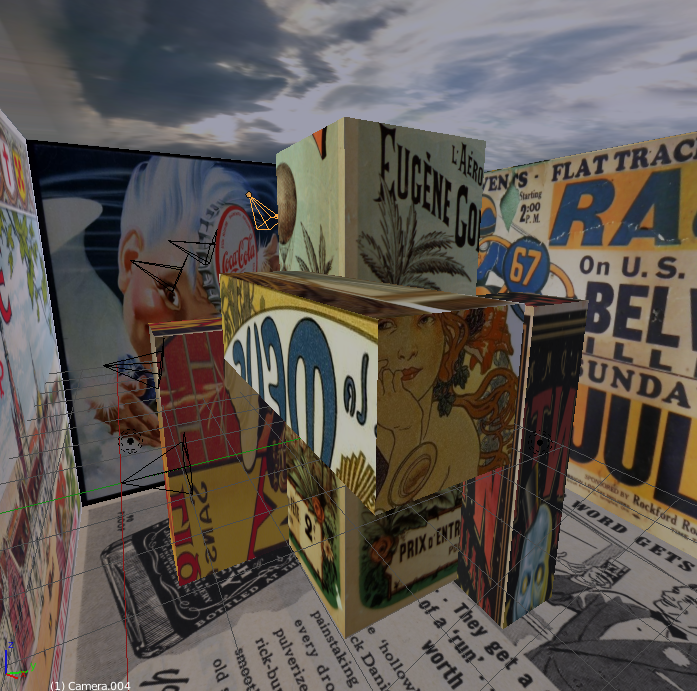
\includegraphics[width=\textwidth]{img/test6_1}
	\end{subfigure}
    %
	\begin{subfigure}{0.4\textwidth}
		\centering
		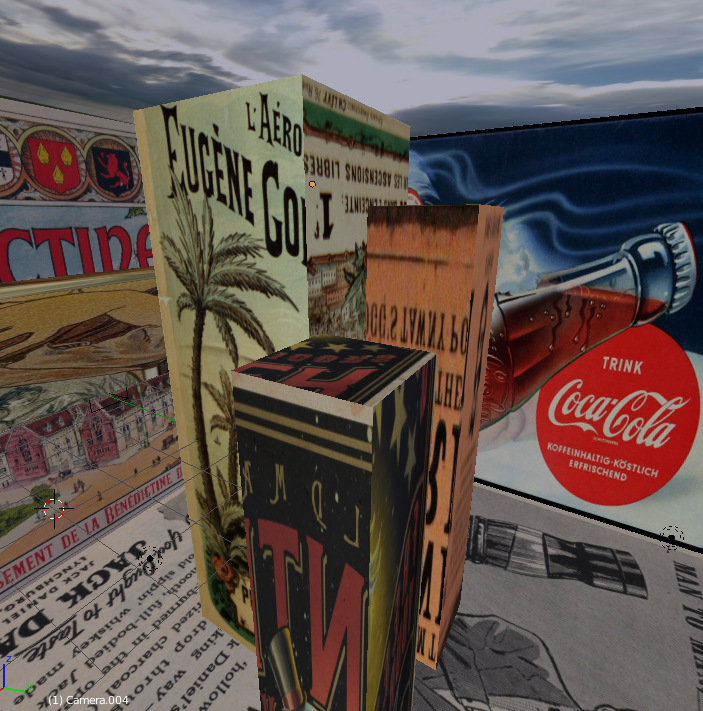
\includegraphics[width=\textwidth]{img/test6_2}
	\end{subfigure}
    %
	\begin{subfigure}{0.4\textwidth}
		\centering
		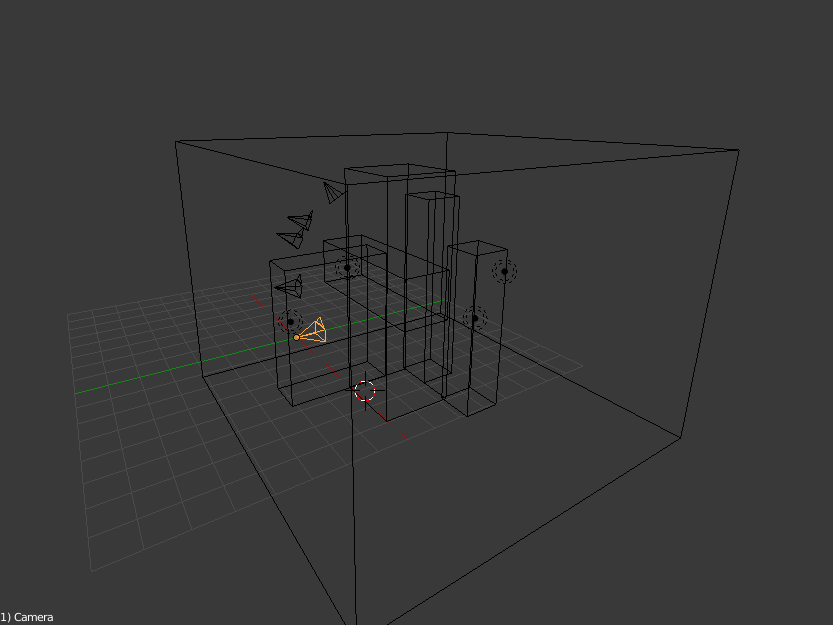
\includegraphics[width=\textwidth]{img/test6_3}
	\end{subfigure}
    %
	\begin{subfigure}{0.4\textwidth}
		\centering
		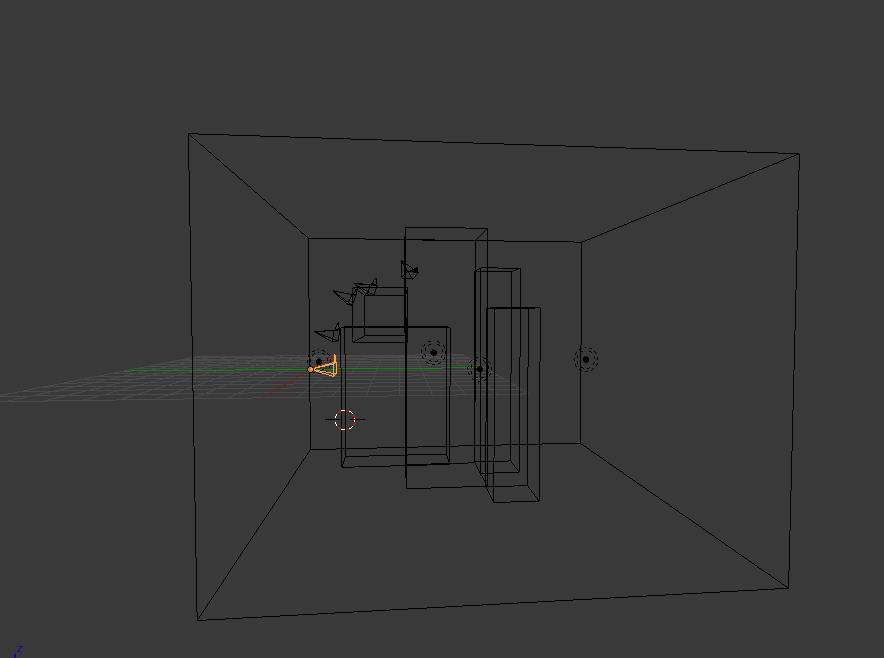
\includegraphics[width=\textwidth]{img/test6_4}
	\end{subfigure}
	%
	\begin{subfigure}{0.8\textwidth}
		\centering
		\includegraphics[width=\textwidth]{img/test6_5}
	\end{subfigure}
	%
	\caption{The first computer-generated environment that we used in our tests and
	an example equirectangular image from this scene: two views of the scene (top row),
	wireframe visualizations of the same scene (middle row), and an example
	equirectangular image produced with this set up (bottom row).}
    \label{fig:test6}
\end{figure}
%

In the second computer-generated scene, we recreated a town square surrounded by
a covered walkway (i.e., \emph{loggia}). The roof of the walkway is supported by columns on the inner
side, the one that is oriented toward the square's centre, and by a wall on the
outer side.
Again the environment is contained in a room and every surface is textured.
The camera moves along the walkway with a non-uniform speed while pointing toward
the centre of the square. Figure~\ref{fig:test_square} shows some images
for this second environment.
%
\begin{figure}
\centering
	\begin{subfigure}{0.4\textwidth}
		\centering
		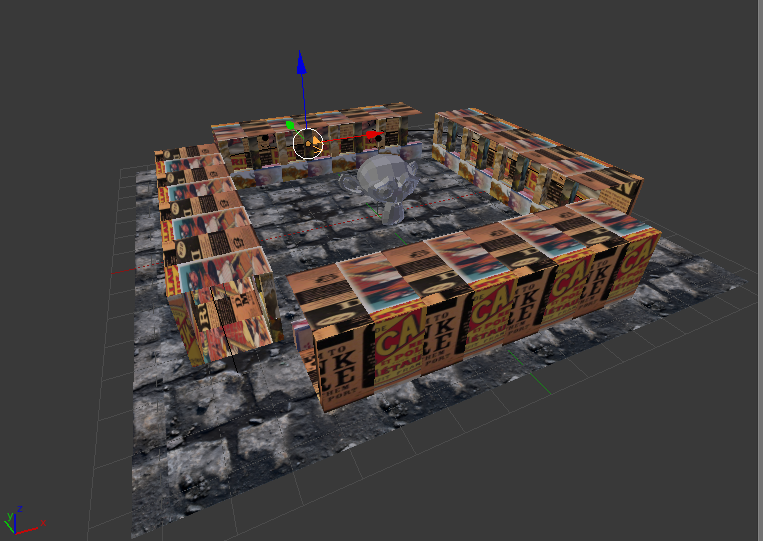
\includegraphics[width=\textwidth]{img/square1}
	\end{subfigure}
    %
	\begin{subfigure}{0.4\textwidth}
		\centering
		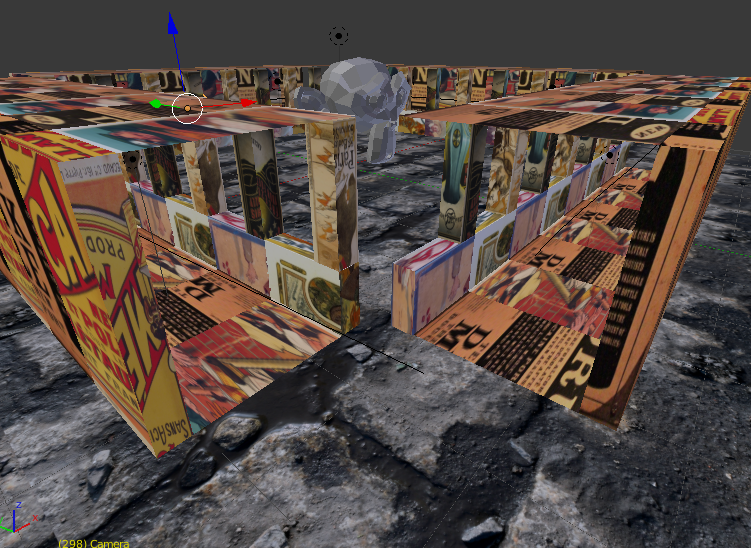
\includegraphics[width=\textwidth]{img/square2}
	\end{subfigure}
    %
	\begin{subfigure}{0.8\textwidth}
		\centering
		\includegraphics[width=\textwidth]{img/square3}
	\end{subfigure}
    %
	\begin{subfigure}{0.8\textwidth}
		\centering
		\includegraphics[width=\textwidth]{img/square4}
	\end{subfigure}
	%
	\caption{The computer-generated town square environment: two views of the
	model (top row) and a two example equirectangular images produced from this
	scene (middle and bottom row).}
    \label{fig:test_square}
\end{figure}

\subsection{Real environment}\label{subsec:real_environment}
We tested our pipeline with a real video footage too. We do not have the ground truth
for the camera poses in the real environment. However, the quality of the
reconstruction is an indicator of the pipeline performance.
We captured the real-world sequence with the Ricoh Theta S camera in a town square
surrounded by a \emph{loggia}. As before, we walked around the square, along the covered
walks, keeping the camera above the user's head using a stick.
The user does not influence the camera poses estimation because it appears in the
pole region of the image sphere and, as we said in
Section~\ref{sec:pipeline_pose_estimation}, we discard potential matches in
these areas.
We present some pictures of the real-wolrd environment together with some examples
of the equirectangular images of the town square in
Figure~\ref{fig:piazzaLeoni}.
%
\begin{figure}[h]
\centering
	\begin{subfigure}{0.7\linewidth}
		\centering
		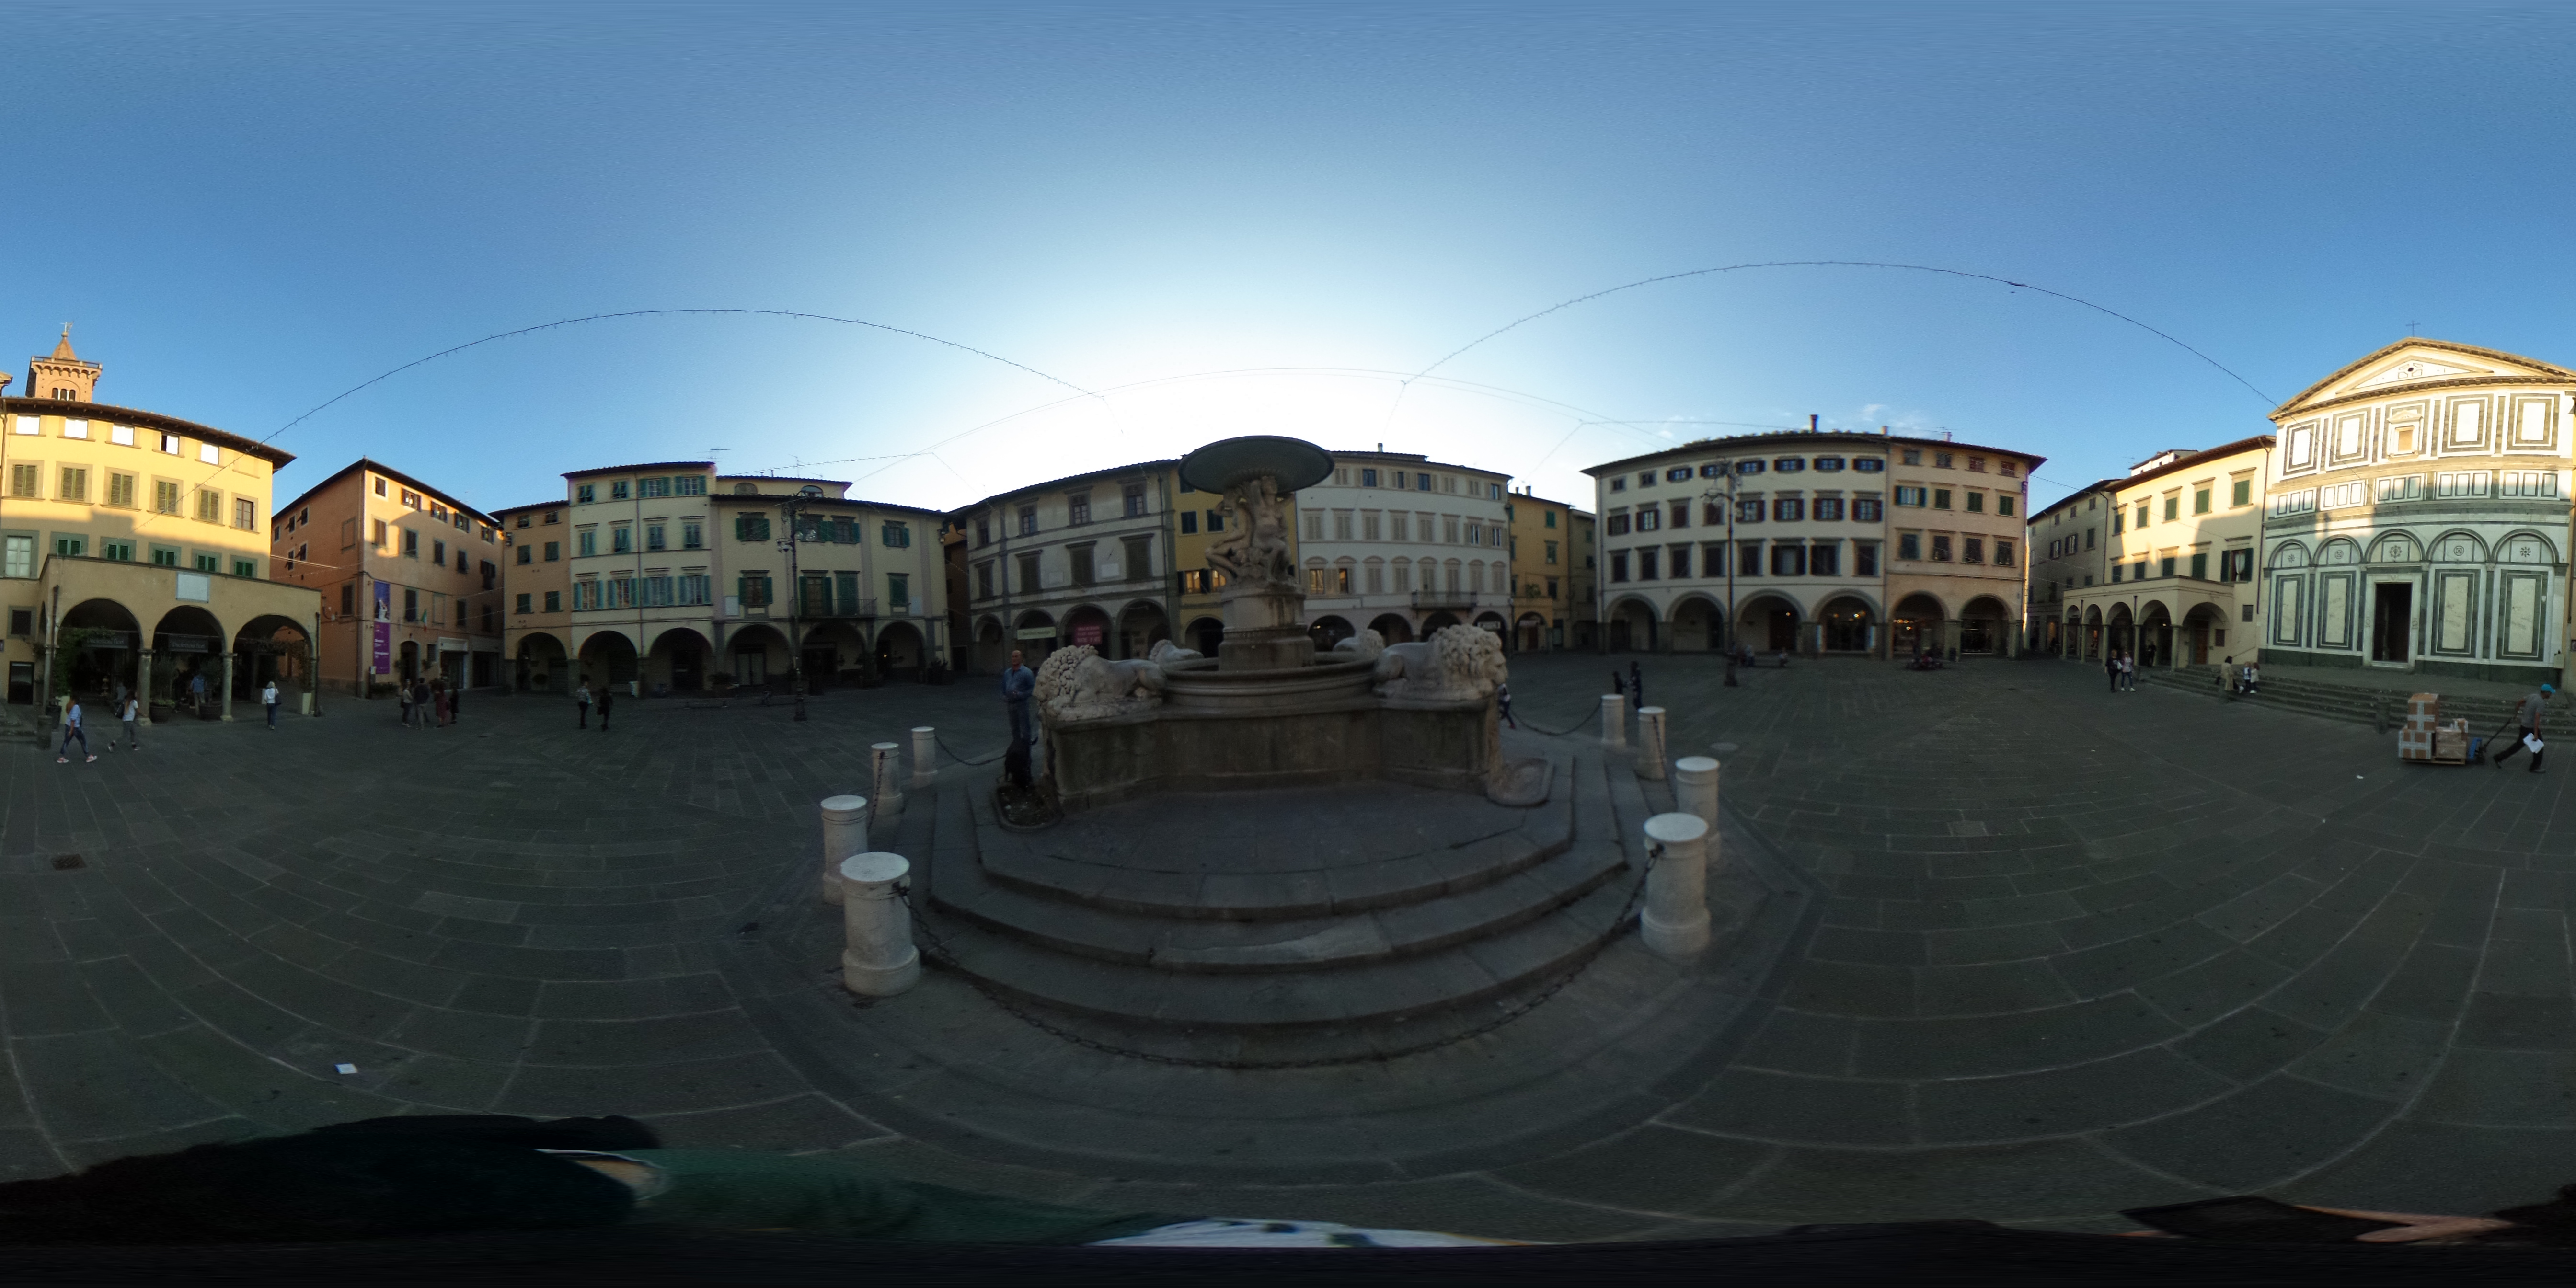
\includegraphics[width=\linewidth]{img/piazzaLeoni.jpg}
		\caption{Panoramic view of the real town square.}
	\end{subfigure}
	%
	\begin{subfigure}{0.7\linewidth}
		\centering
		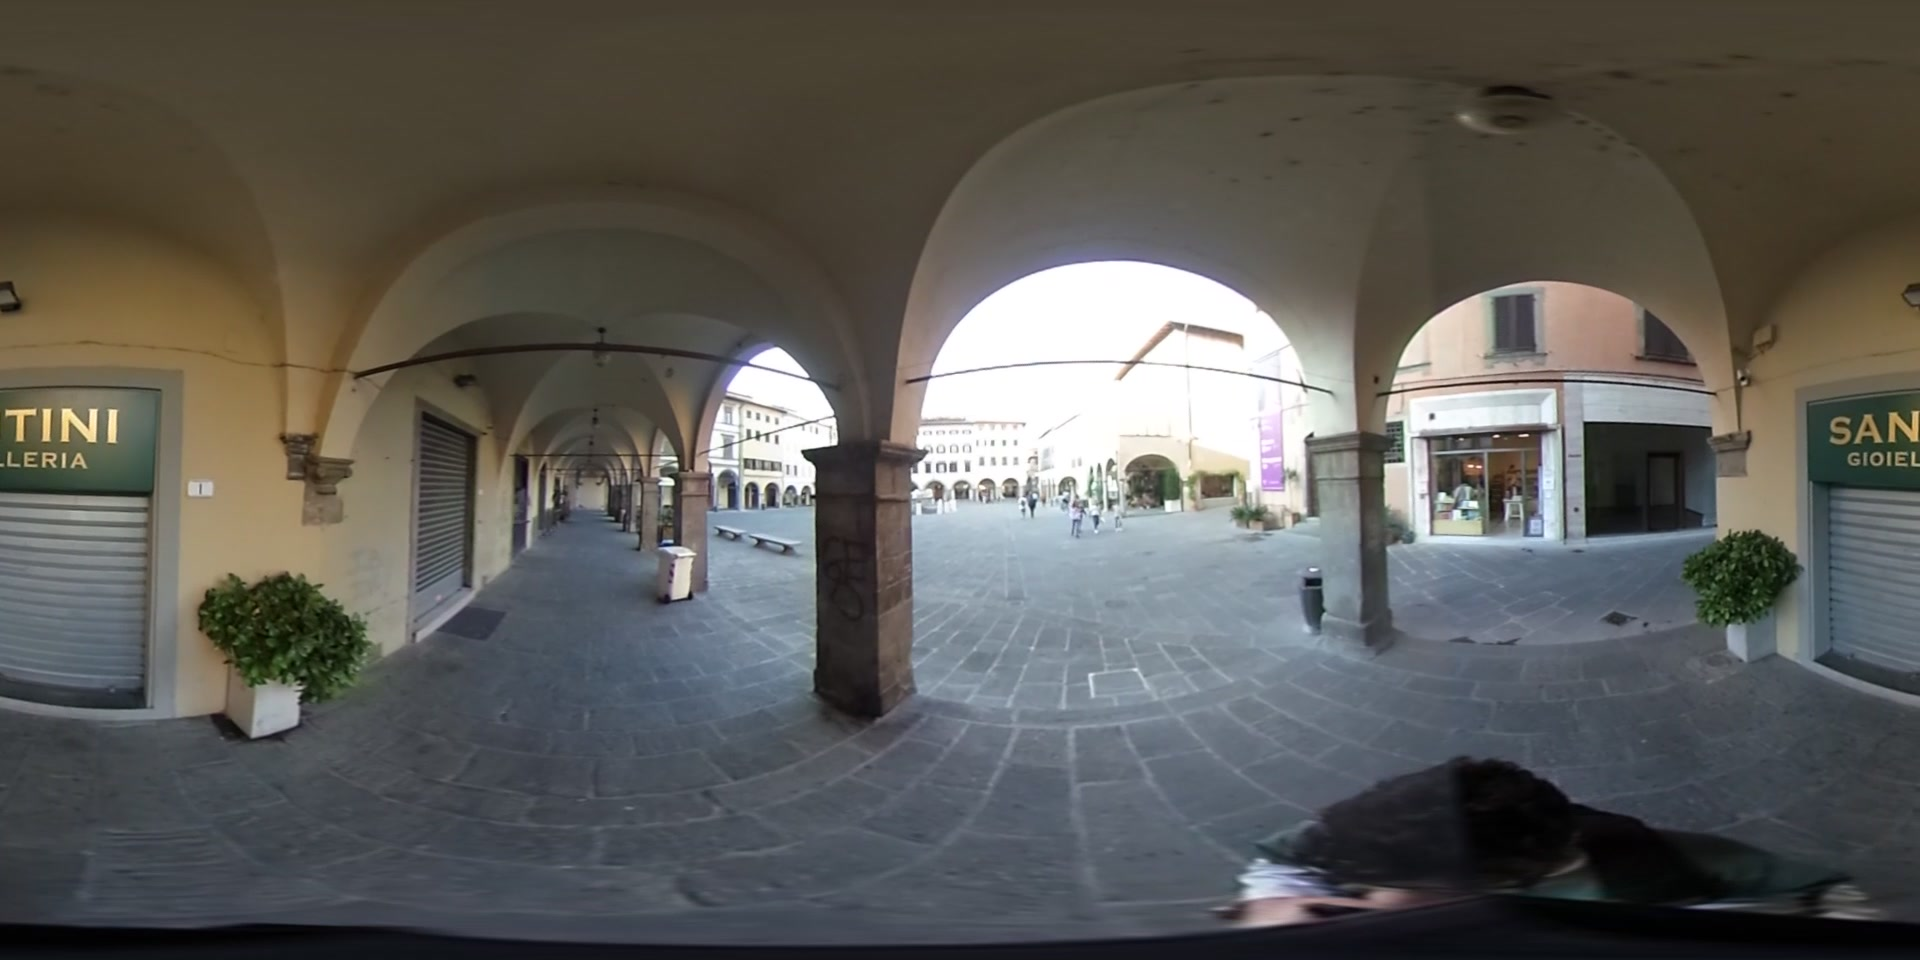
\includegraphics[width=\linewidth]{img/piazzaLeoni_exampleds.jpg}
		\caption{Example frame from the real town square sequence.}
	\end{subfigure}
\caption{The town square we used in our real-world reconstruction test.}
\label{fig:piazzaLeoni}
\end{figure}

\section{Experiment Results}
\subsection{Window Size Test}
We performed an experiment to choose the optimal window size for the windowed
bundle adjustment (Section~\ref{subsec:windowed_ba}). In this experiment, we
used the synthetic town square and computed the sum of absolute pose error. In
particular, we found the location and orientation errors for the estimated poses.
Figure~\ref{fig:sumAbsLocError} shows the comparison of the resulted location error for 20
estimated poses with respect to several windowed and non-windowed adjustment
techniques.
In particular, we can see that the pose error is minimal when we employ the
windowed bundle adjustment with a window that contains five poses at a time.
Windows smaller than five do not bring substantial improvements (as we pointed out in
Section~\ref{subsec:windowed_ba}; to maintain the proper scale, we keep the two poses
in a window fixed), while the error also increases
for larger windows. The performance deterioration when using larger windows
is due to the fact that the windowed adjustment may suffer from the high number
of views to be optimized: if a series of views with wrong estimated poses are
already inside the window and a new pose enters it, the prevalent number of
low-quality estimation may result in the last pose to be aligned to the wrong trajectory
of the previous estimations. Due to this phenomenon, all next views
may be incorrectly optimized. This reduces the performance of the overall
pose estimation.
%
\begin{figure}[h]
\centering
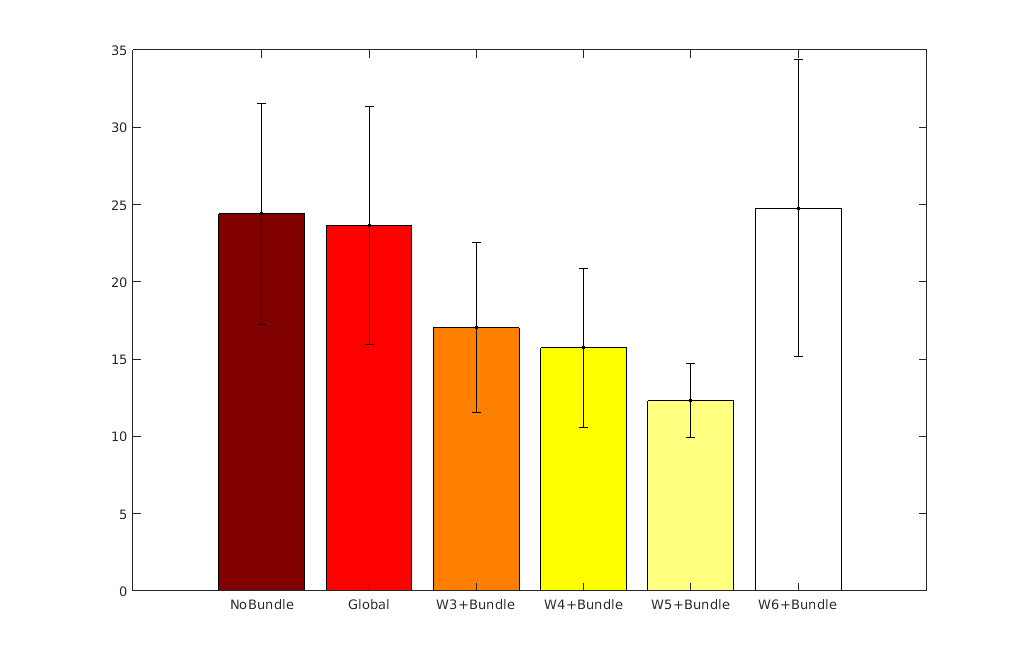
\includegraphics[width=\linewidth]{img/sumAbsLocError.png}
\caption{How the location error varies with respect to the adjustment technique
used. Angular errors present a similar behaviour with a minimum in case
of windowed bundle adjustment whose window length set to five views.}
\label{fig:sumAbsLocError}
\end{figure}

\subsection{Essential Matrix Estimation Test}\label{subsec:essential_test}
In Section~\ref{subsec:essential_estimation}, we said that our pipeline
calls the essential matrix estimation routine until the fraction of inliers
drops below a threshold. In Figure~\ref{fig:essential_test}, we show the
results of an experiment where we compare three different essential matrix
evaluation approaches. The input data for this experiment is composed of
a set of manually selected frames from the first synthetic environment.
The reason why we select the frames is that we do not want this results to be
influenced by the frame filter.
%
\begin{figure}[h]
\centering
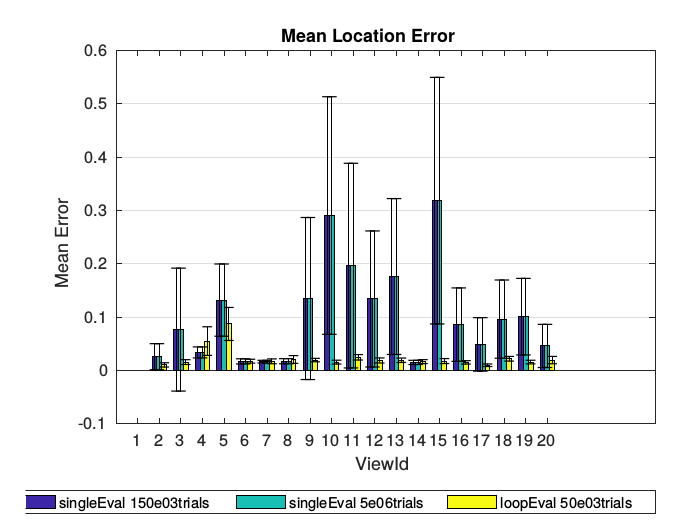
\includegraphics[width=\linewidth]{img/essentialEstimation.png}
\caption{How the location error changes with respect to different essential
matrix estimation function approaches: the purple and light blue columns
represent the average location error results for each frame when the
essential estimation is performed with a single call to the routine, while the
yellow column represent the location error when we perform the estimation
again when the fraction of inliers is too low.}
\label{fig:essential_test}
\end{figure}

\subsection{SfM Phase Result}
In this test, we analyzed the overall results of the initial step of our
pipeline, the motion estimation phase. We used the 365 rendered frames of our
synthetic town square environment. Figure~\ref{fig:trajectory} shows the actual
and estimated trajectory of the camera in the synthetic environment.
%
\begin{figure}[h]
\centering
\begin{subfigure}{0.45\linewidth}
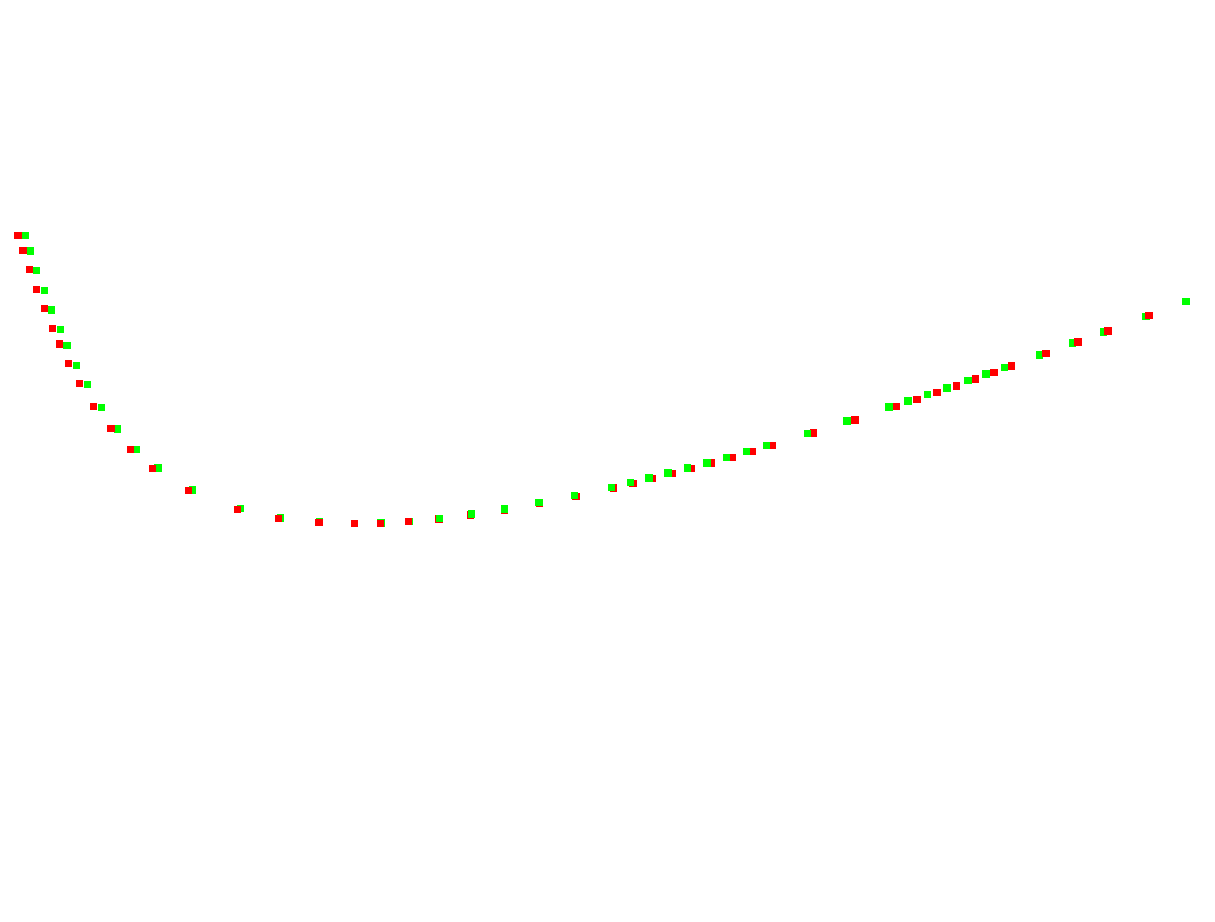
\includegraphics[width=\linewidth]{img/snapshot00.png}
\label{fig:trajectory1}
\end{subfigure}
\begin{subfigure}{0.45\linewidth}
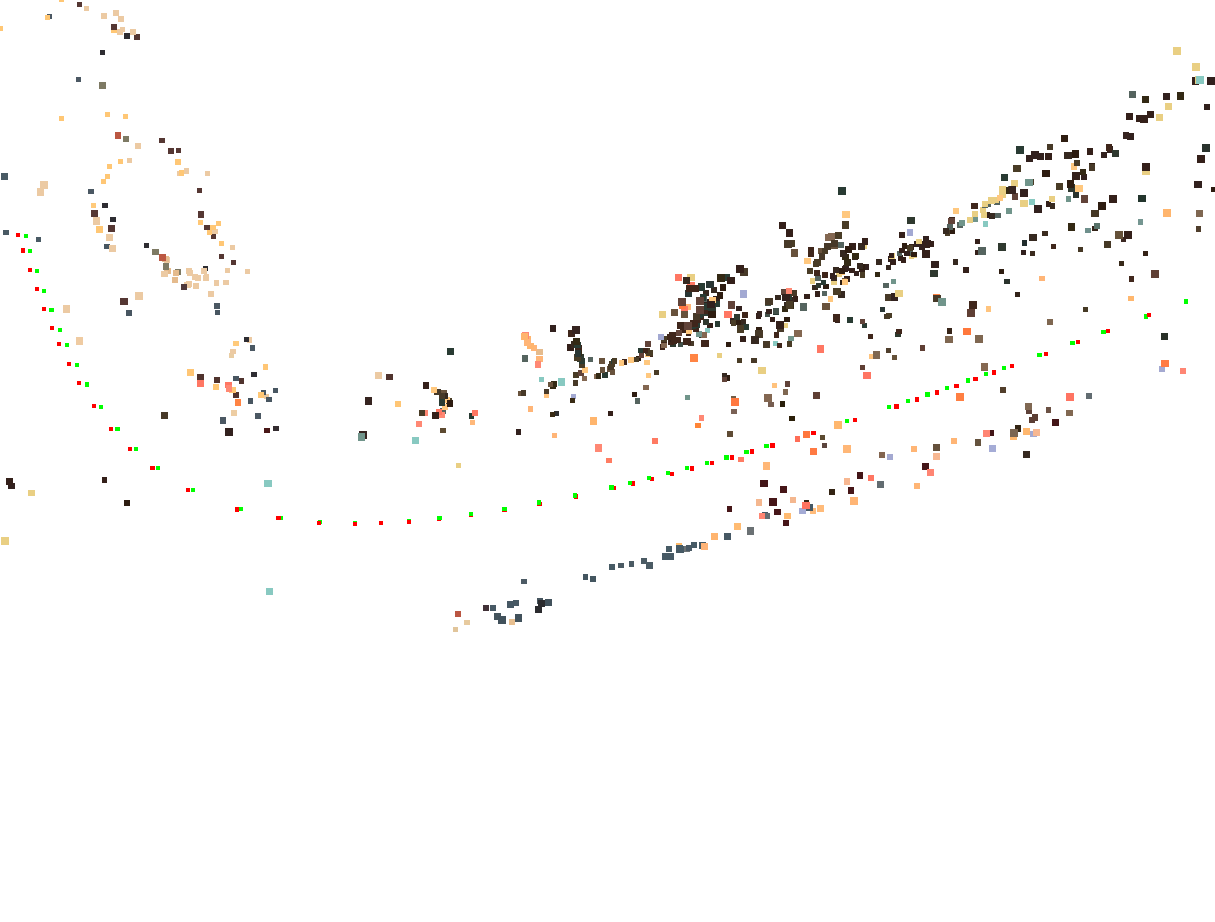
\includegraphics[width=\linewidth]{img/snapshot01.png}
\label{fig:trajectory2}
\end{subfigure}
\begin{subfigure}{\linewidth}
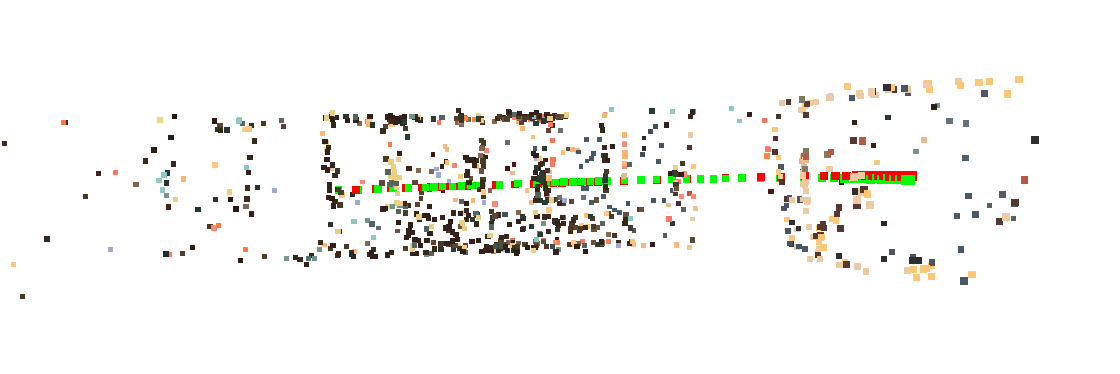
\includegraphics[width=\linewidth]{img/snapshot02.png}
\label{fig:trajectory3}
\end{subfigure}
\caption{The results of the pose estimation phase: estimated poses (green
points) compard with ground truth (red points) (a); the sparse point cloud
composed of the triangulated features points (b); another view of the sparse
point cloud where we can distinguish the columns of the inner side of the
walkway (c).}
\label{fig:trajectory}
\end{figure}
%
\subsection{Disparity Maps}
Figure~\ref{fig:llDisparity} shows an example of disparity map computed
with our adaptive block-matching algorithm. Darker colours refer to the points
with less disparity thus, farther from the camera. On the other hand, the closer
objects have brighter colours.
%
\begin{figure}[h]
\centering
	\begin{subfigure}{0.7\linewidth}
		\centering
		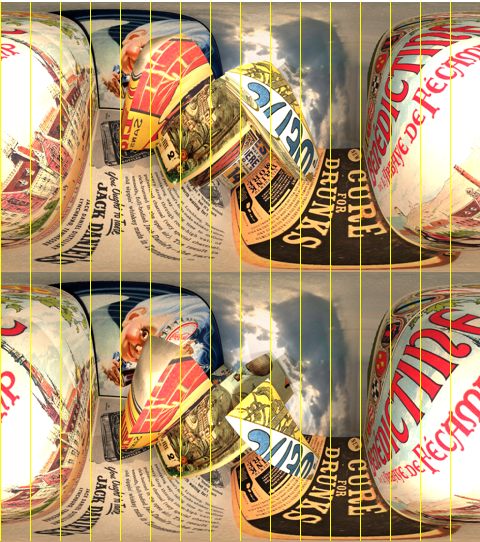
\includegraphics[width=\linewidth]{img/rectified_pair.png}
		\caption{Original rectified pair.}
	\end{subfigure}
	%
	\begin{subfigure}{0.7\linewidth}
		\centering
		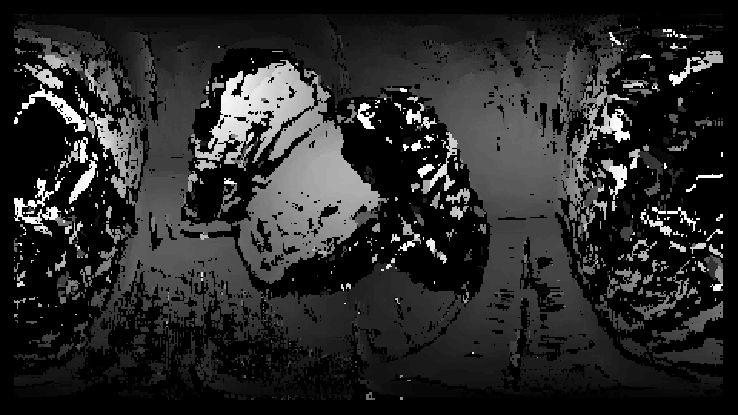
\includegraphics[width=\linewidth]{img/lldisparity2.png}
		\caption{Computed disparity map.}
	\end{subfigure}
\caption{An example of disparity map computed with our adaptive block-matching
algorithm. The black point in the map are points whose disparity is equal to
zero or that are occluded in the other image; in both cases, these points are
not triangulated.}
\label{fig:llDisparity}
\end{figure}

\subsection{Environments Reconstruction}
Figure~\ref{fig:real_reconstruction} shows the resulting reconstruction of the
real town square's loggia described in Section~\ref{subsec:real_environment}.
%
\todo[inline]{Questa ricostruzione e' solo una prova limitata a 4 coppie di view.}
\begin{figure}[h]
\centering
	\begin{subfigure}{0.45\linewidth}
		\centering
		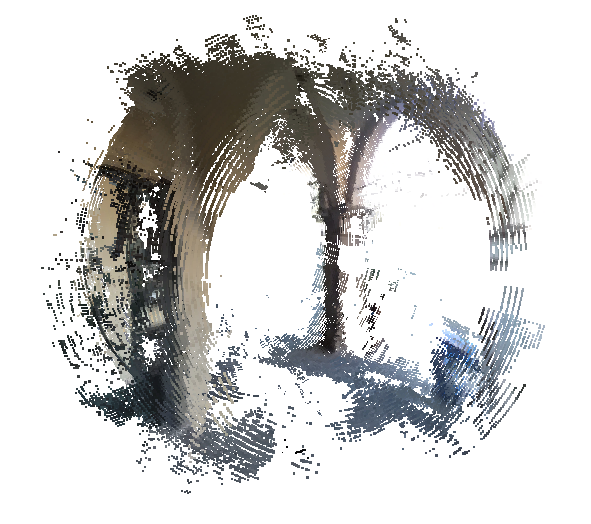
\includegraphics[width=\linewidth]{img/reconstruction1.png}
	\end{subfigure}
	%
	\begin{subfigure}{0.45\linewidth}
		\centering
		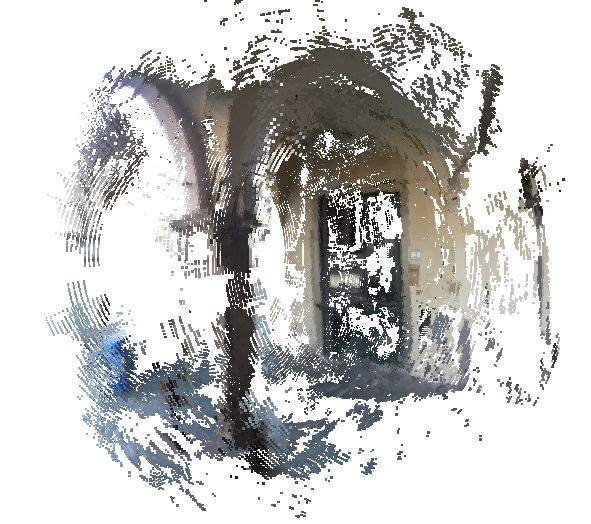
\includegraphics[width=\linewidth]{img/reconstruction2.png}
	\end{subfigure}
	\caption{Two views of the dense point cloud of the real town square
	(Section~\ref{subsec:real_environment}) obtained with our SfM pipeline.}
	\label{fig:real_reconstruction}
\end{figure}

\chapter{Conclusion}
\lhead{\chaptername~\thechapter. \emph{Conclusion}}
%
\section{Future Work}\label{sec:future_work}
Our SfM pipeline employs existing correspondences between adjacent frames only.
This is because we use video sequences as input data, thus the presence of
the same features of the current frame in the next one is a natural consequence
of the particular nature of our input.
As we pointed out in Section~\ref{subsec:limitations}, this particular choice
for feature matching can be a problem when not enough feature points can be
tracked in all the views of the window.
The current implementation of our pipeline does not deal with this problem,
hence, it is up to the user to remove the responsible frames and produce two
separate reconstruction instead that can later be merged.
This split-reconstruct-merge workaround can be automatized by using SLAM's
loop-closure detection (Section~\ref{sec:sfm_vo_slam}).
Loop closure is the process of detecting the camera crossing a previously
visited place, thus it can detect when separate trajectories intercept
and automatically merge the camera's paths and create single reconstruction.

The inclusion of a more powerful \emph{scene-graph} is a possible improvement
whose potential benefits can be investigated in the future.
A scene graph can improve the pose estimation
performance by introducing additional redundant data derived by 
correspondences matching between pairs of non-consecutive images.
A more robust features detection and matching for highly distorted images
can improve the quality of local motion estimation by increasing the number
of both detected and correctly matched features of image pairs.
Some of the possible alternative algorithms are ASIFT~\cite{morel2009asift}, which
 can perform better in case of views with very tilted cameras, and
BRISKS~\cite{guan2017brisks}, a feature detector inspired by
BRISK~\cite{leutenegger2011brisk} and designed specifically for full spherical
images.
Another approach to improve local motion estimation is to
introduce a procedure to extract
features that are evenly distributed across an image. The more
keypoints are spread over an image, the more accurate is the local motion
estimation~\cite{irschara2009structure,schonberger2016structure}.

A future implementation of our pipeline is already planned; it will contribute
to possible improvement with a procedure to extract features uniformly
distributed across an image sphere. \todo{Chiedere se c'e' un paper da citare}

\section{Conclusion}
In this work, we have proposed a SfM pipeline for full spherical cameras.
As we pointed out in Section~\ref{sec:contribution} and
Section~\ref{subsec:related_work}, our contribution includes:
%
\begin{itemize}
	\item a novel frame filter that selects frames based on visual
	information only;
	\item a new approach to estimate poses that exploits both frontal and rear
	points;
	\item a novel block-matching algorithm for disparity map estimation from
	equirectangular images.
\end{itemize}
%
We have showed the effectiveness of our pipeline by testing it on 
both computer-generated and real-world environments.
Even though our approach is extremely straightforward, especially when compared to more advanced pipeline (e.g.,~\cite{schonberger2016structure}, it still offers high-quality results in terms of
poses estimation precision and environment reconstruction.


\clearpage
\lhead{\emph{\bibname}}
\printbibliography

\end{document}
